\section{Data Cleaning}\label{app:MLDataCleaning}

% number of missing obs?

% no invalid long, lat values
% no speed values above 30 knots (according t Oliver)
% implied speed?
% Source: AIS_Calculations.py

% Jumps
% greater than 170 above 5 knots or 
% Source: AIS_Calculations.py

% number of impossible values?
% number of jumps?
% number of drafts infilled?

% After interpolation
% high speed values!
% high distance values

\section{Summary Statistics}\label{app:summarystats}

% representativeness of EU MRV reporting fleet
% mean, sd of all variables

\section{Trip Detection}\label{app:tripdetection}


\section{Machine Learning Details}\label{app:mldetails}

The optimal tuning parameters are provided in \autoref{tab:trainparams}.
\begin{table}[H]
    \centering
    \begin{adjustbox}{max width=\textwidth}
    \begin{threeparttable}
        \caption{Optimal tuning parameters}
        \label{tab:trainparams}
        
\begin{tabular}[t]{llr}
\toprule
\multicolumn{1}{l}{Model} & \multicolumn{1}{l}{Parameter} & \multicolumn{1}{l}{Value}\\
\midrule
 & depth & 6\\

 & l2 leaf reg & 1\\

\multirow[t]{-3}{*}{\raggedright\arraybackslash CatBoost Regressor} & learning rate & 0.1\\
\cmidrule(lr){1-3}

 & learning rate & 0.01\\

\multirow[t]{-2}{*}{\raggedright\arraybackslash Gradient Boosting Regressor} & max depth & 3\\
\cmidrule(lr){1-3}

Lasso & alpha & 0.005\\
\cmidrule(lr){1-3}

Linear Regression & n/a & n/a\\
\cmidrule(lr){1-3}

 & max depth & 50\\

\multirow[t]{-2}{*}{\raggedright\arraybackslash Random Forest Regressor} & n estimators & 200\\
\cmidrule(lr){1-3}

Ridge Regression & alpha & 10\\
\bottomrule
\end{tabular}

        % \begin{tablenotes}[flushleft]\small
            % \item \textit{Note:} MAE is mean absolute error, and $R^2$ is the coefficient of determination. The best score for each metric is highlighted in bold.
        % \end{tablenotes}
    \end{threeparttable}
    \end{adjustbox}
\end{table}

The inferior performance of the CatBoost model versus ridge regression is shown in \autoref{fig:twoway_test_compare2_levels}.
\begin{figure}[H]
    \centering
    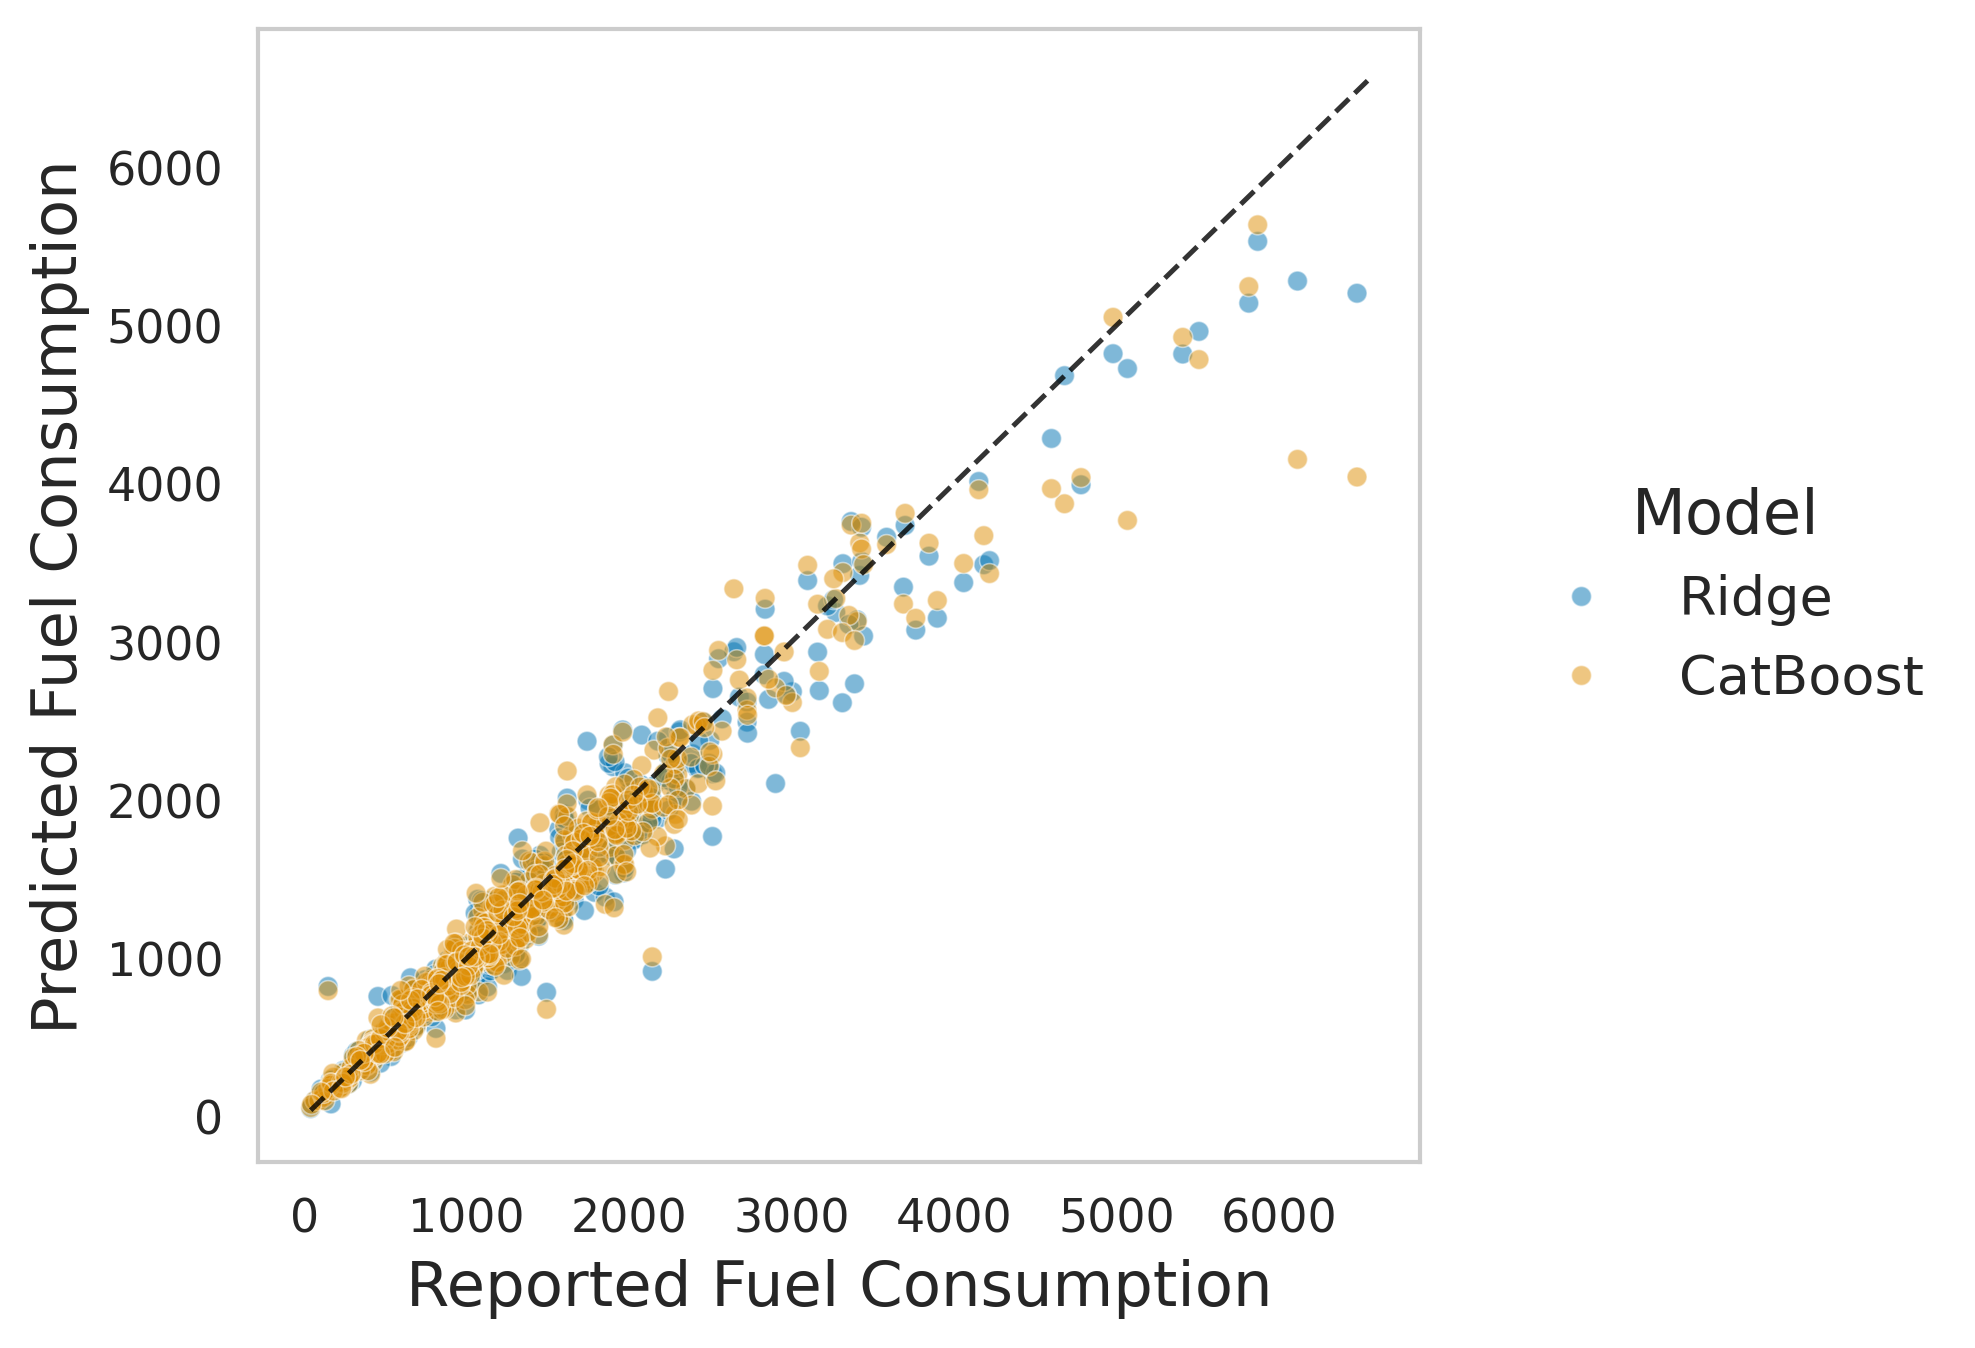
\includegraphics[width=0.65\textwidth]{ML_FC_Fm5dd_twoway_test_levels_compare2.png}
    \caption{Test set prediction accuracy (levels) for ridge regression and CatBoost}
    \label{fig:twoway_test_compare2_levels}
\end{figure}

\section{Alternative Data Inclusion Criteria}\label{app:altcriteria}